% !Mode:: "TeX:UTF-8"
%%  本模板推荐以下方式编译:
%%     1. PDFLaTeX[推荐]
%%     2. xelatex [含中文推荐]
%%  注意:
%%  1. 文件默认的编码为 UTF-8 对于windows,请选用支持UTF-8编码的编辑器。
%%   2. 若是模板有什么问题,请及时与我们取得联系,Email:latexstudio@qq.com。
%%   3. 可以到  https://ask.latexstudio.net 提问
%%   4. 请安装 最新版本的 TeXLive 地址:
%%   http://mirrors.ctan.org/systems/texlive/Images/texlive.iso

\documentclass{apmcmthesis}

\usepackage{url}

%%%%%%%%%%%%填写相关信息%%%%%%%%%%%%%%%%%%%%%%%%%%
\tihao{C}                            %选题
\baominghao{apmcm2300201}                 %参赛编号
\begin{document}

\pagestyle{frontmatterstyle}

\begin{abstract}
% using \CJK{UTF8}{gbsn}{Chinese} for Chinese.

New energy vehicles have gained widespread popularity since their introduction, due to their advanced technology, low fuel consumption, and alignment with the global carbon peak and carbon neutrality goals around the world. This paper extensively gathers data on new energy vehicles, traditional fuel-powered cars, and related information. Finally, a series of mathematical models to describe the development of new energy vehicles are established.

For problem 1, 

For problem 2, the sales data for China's new energy electric vehicles over the last decade, along with the sales data for all vehicles in China over the past twenty years, have been collected. Using this data, an ARIMA model was established. By forecasting the sales changes for the next ten years for both new energy electric vehicles and all vehicles, we've analyzed the future development of China's new energy electric vehicles for the upcoming decade. 

For problem 3, by analyzing the impact of China's new energy electric vehicle development on traditional vehicles sales in China, the impact of new energy electric vehicle development on the global traditional automotive industry can be reflected. The Pearson correlation coefficient was employed to calculate the correlation between China's new energy electric vehicle sales and traditional car sales in China.

For problem 4,

For problem 5,

For problem 6,

Ultimately, we provide a summary of the data and mathematical models employed in this study and look ahead to potential future works.


\keywords{New energy vehicles\quad  Principal Component Analysis\quad   ARIMA\quad   Pearson correlation\quad    Multiple Linear Regression}
\end{abstract}


\newpage
%目录
\tableofcontents


\newpage
\pagestyle{mainmatterstyle}
\setcounter{page}{1}
\section{Introduction}

% 首先写新能源汽车的意义(总体介绍)

% 然后写新能源汽车对中国的特殊意义和在中国的发展
% 以及新能源电动汽车(题目只涉及新能源电动汽车)

% 最后写本文的做法(建模主体即:中国、新能源电动汽车)

New energy vehicles integrate transformative technologies such as new energy sources, new materials, and various disruptive technologies like the internet, big data, and artificial intelligence. This integration propels the transformation of energy, transportation, and information communication infrastructure, fostering an optimized energy consumption structure, elevating the intelligence level of transportation systems and urban operations. This advancement holds significant importance in constructing a clean and beautiful world, and in building a shared future for humanity.

The widespread adoption of new energy vehicles holds particular significance for China. With a large population, China faces substantial carbon emissions from automobiles. The popularization of new energy vehicles will greatly reduce China's energy expenditure and stands as a robust initiative toward achieving ecological civilization.

Within the realm of new energy vehicles, the development of new energy electric vehicles has been particularly rapid. This is primarily due to their low pollution and low energy consumption characteristics. Additionally, new energy electric vehicles typically offer a affordable price, thus enjoying a broad market in China.

This paper collects comprehensive data on China's new energy electric vehicles, including their sales volume, growth rates, traditional car sales, export quantities, and China's policies supporting new energy vehicles. Further, this paper employs methods such as \textbf{xx} and \textbf{xx} to model and analyze the development of China's new energy electric vehicles and their associated impacts.


\section{The Description of the Problem}

In this chapter, we conducted a detailed analysis of six problems related to the development of new energy vehicles and provided approaches to address these problems.

\subsection{Question 1}

Firstly, the development of China's new energy electric vehicles is assessed through their sales volume. While numerous factors influence the development of China's new energy electric vehicles, some of the factors like policies and scientific technologies cannot be quantified, hence making them unsuitable for mathematical modeling. Therefore, factors can be quantified such as household income and gasoline prices are selected as factors. Principal component analysis (PCA) is employed to analyze the main factors affects the sales volume of China's new energy electric vehicles, i.e., the development of China's new energy electric vehicles.

\subsection{Question 2}

Similar to the first inquiry, we continue to utilize the sales volume of China's new energy electric vehicles as a measure of their development. To forecast the development of new energy electric vehicles over the next decade, we employ past sales data of new energy electric vehicles and all vehicles to predict the sales of new energy electric vehicles and all vehicles for the next ten years, which aims to examine their growth trajectory. This problem is modeled as a time series prediction problem, and we employ Autoregressive Integrated Moving Average (ARIMA) model to address the problem.

\subsection{Question 3}


The market share of China's automotive industry is substantial on a global scale. Hence, this paper uses the development of new energy electric vehicles in China as a reflection of the global progress in this sector, while the traditional automotive industry in China mirrors the global traditional automotive industry. Furthermore, this study continues to utilize the sales figures of new energy electric vehicles and cars in China to represent their respective developments. Thus, this issue is modeled as the impact of sales of new energy electric vehicles in China on the sales of traditional vehicles in China. Correlation analysis is deployed to describe the impact of new energy vehicles on traditional vehicles.

\subsection{Question 4}



\subsection{Question 5}



\subsection{Question 6}




\section{Models}

\subsection{Model for Question 1}

\subsubsection{Terms, Definitions and Symbols}
\% introduce $Terms, Definitions, Symbols$ used in this model.



\subsubsection{Assumptions}


\subsubsection{Data preparation}


\subsubsection{The Foundation of Model}
\% Establish mathematical model here.


\subsubsection{Solution and Result}
\% Solve mathematical model here.


\subsubsection{Analysis of the Result}
\% Conclude here.


\subsubsection{Strength and Weakness}
\% Optional
\begin{description}
\item[Strength:] Strength.
\item[Weakness:] Weakness.
\end{description}


\subsection{Model for Question 2}

\subsubsection{Terms, Definitions and Symbols}

The Symbols used in this section will be demonstrated right following its use.

\subsubsection{Assumptions}

Our objective is to forecast the next decade's sales of new energy electric vehicles based on past sales data and similarly predict the next ten years' sales of all vehicles using previous sales data. Therefore, we assume a certain pattern within the vehicle sales data, suggesting that future data can be forecasted based on prior trends.

\subsubsection{Data preparation}

Our collected sales data for new energy electric vehicles and all vehicles are illustrated in Figure \ref{figure 1}. In Figure \ref{figure 1}, the red line represents the curve of total car sales over time, while the blue line represents the curve of new energy electric vehicle sales over time. The horizontal axis denotes time, and the vertical axis represents sales (in units of ten thousand vehicles).

Within the sales data for new energy electric vehicles, there are instances of missing data. Upon observation, the missing data segments exhibit minimal fluctuations. Hence, we have opted to employ linear interpolation to fill in the gaps within the data. Linear interpolation used in our process to fill in the gaps within the data is formulated as:

\begin{equation}
	\hat{y} = y_s + (y_e - y_s) \times \frac{y_e - y_s}{x_e - x_s}
\end{equation}

where $\hat{y}$ is the predicted value of the missing data in position $x$, $y_e$ is the ending $y$ value of the missing data segment, $y_s$ is the starting $y$ value of the missing data segment, $x_e$ is the ending $x$ value of the missing data segment, $x_s$ is the starting $x$ value of the missing data segment.

The interpolated data is shown in Figure \ref{figure 2}. With interpolated data, ARIMA model can be deployed to time series prediction task.

\begin{figure}[htbp]
	\centering
	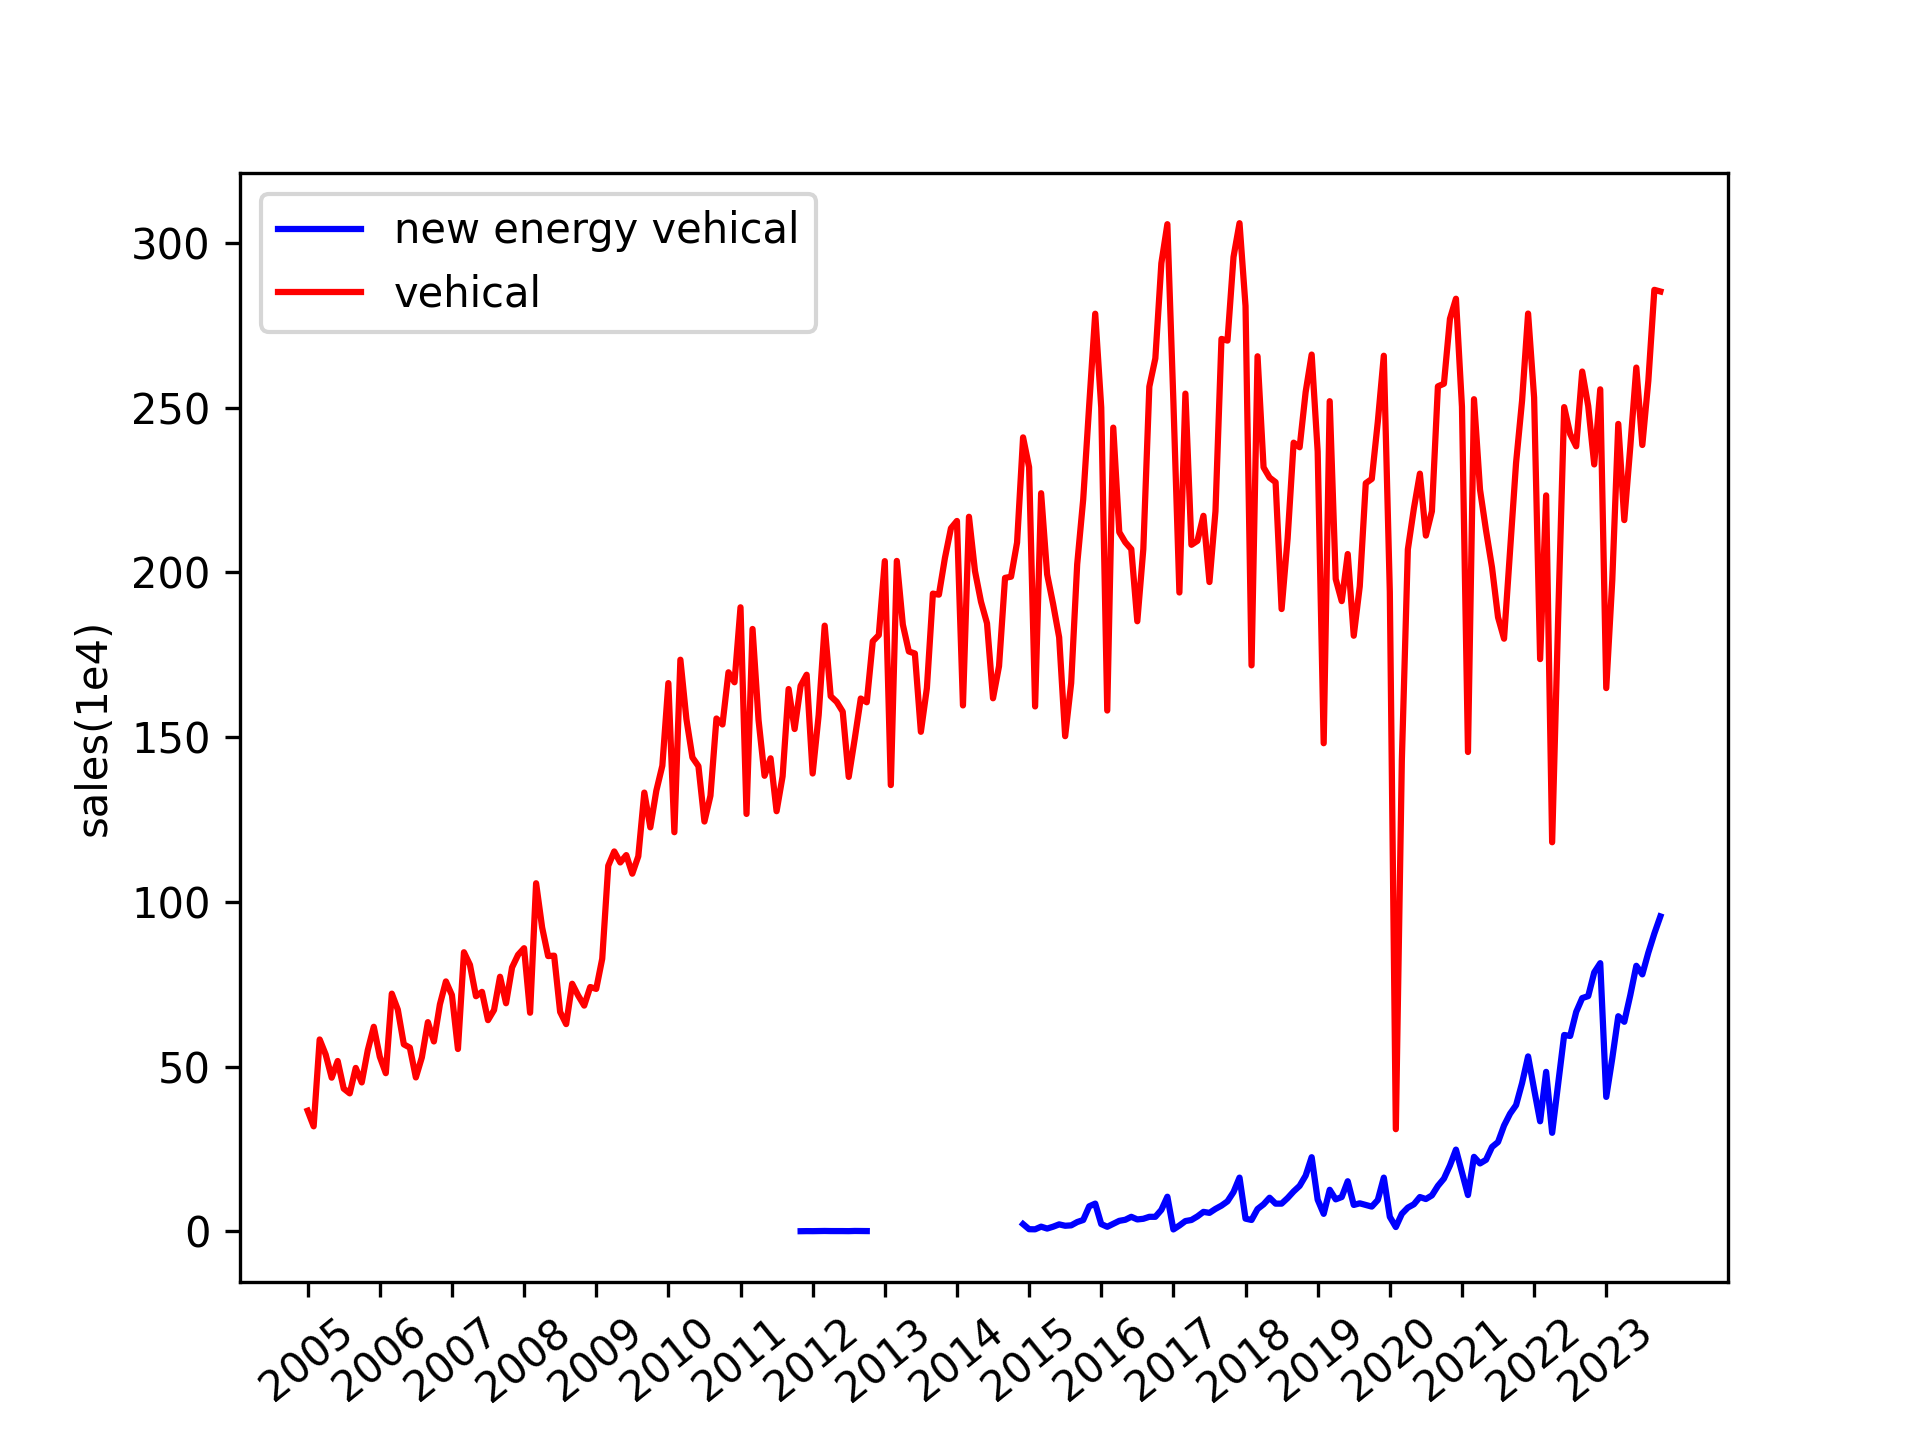
\includegraphics[width=30pc, height=22pc]{origin_new_energy_data}
	\caption{Original data.}
	\label{figure 1}
\end{figure}

\begin{figure}[htbp]
	\centering
	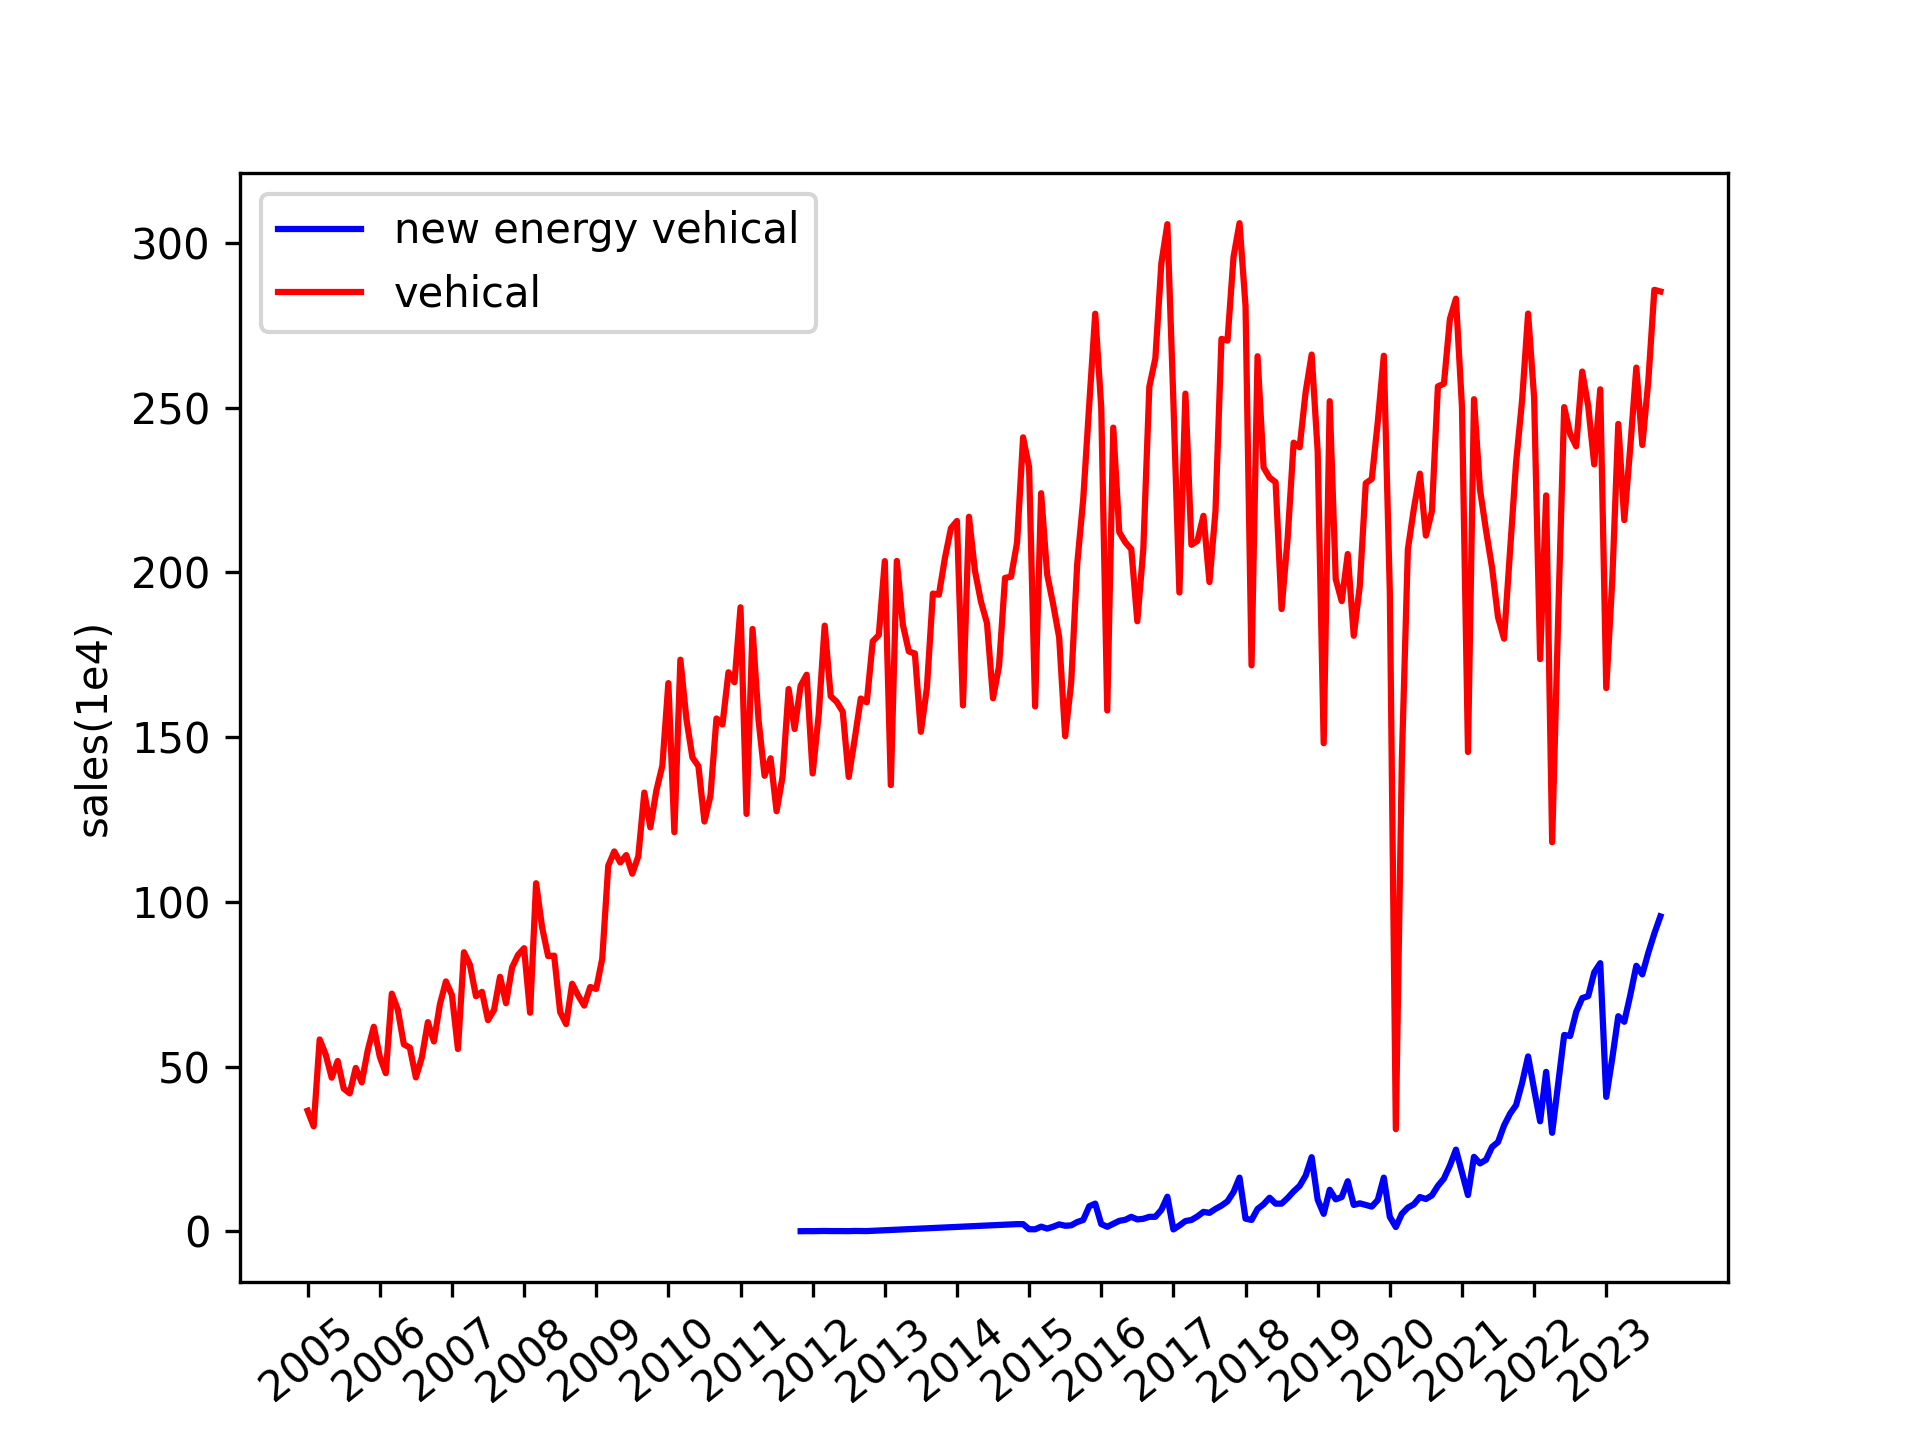
\includegraphics[width=30pc, height=22pc]{interpolated_new_energy_data}
	\caption{Processed data.}
	\label{figure 2}
\end{figure}


\subsubsection{The Foundation and Solution of Model}

The modeling process with ARIMA model is described as:

\textbf{Step1:} Stationarity Check: Assess the stationarity of the time series data by examining mean, variance, and autocorrelation structure.

\textbf{Step2:} Differencing: If the data is non-stationary, perform differencing to achieve stationarity. This involves computing differences between consecutive observations.

\textbf{Step3:} Identify Parameters: Determine the parameters of the ARIMA model—p (autoregressive order), d (degree of differencing), q (moving average order)—through autocorrelation and partial autocorrelation function plots.

\textbf{Step4:} Fit the Model: Fit the ARIMA model to the stationary data by selecting appropriate values for p, d, and q.

Overall, the ARIMA model consists of three parts: differencing, autoregression, and moving average. Differencing eliminates non-stationarity in the data by computing the differences between current and previous values. This step is achieved through the application of differencing operations. Its formula is:

\begin{equation}
	(1 - B)^d \cdot Y_t = \varepsilon_t
\end{equation}

where $\varepsilon_t$ represents the white noise error term, $B$ is the differencing operator, and $d$ represents the number of differencing iterations. 

The autoregressive component describes the relationship between current and previous values. The mathematical expression for the AR part is as follows:

\begin{equation}
	\phi_p \cdot y_{t-p} + \phi_{p-1} \cdot y_{t-(p-1)} + \ldots + \phi_1 \cdot y_{t-1} = \varepsilon_t
\end{equation}

where $\phi$ represents the autoregressive coefficient, and $p$ denotes the autoregressive order.

The moving average component describes the relationship between the current value and the random error terms. The mathematical expression for the MA part is as follows:

\begin{equation}
	\varepsilon_t = \theta_q \cdot \eta_{t-q} + \theta_{q-1} \cdot \eta_{t-(q-1)} + \ldots + \theta_1 \cdot \eta_{t-1}
\end{equation}

where $\theta$ signifies the moving average coefficient, $q$ denotes the moving average order.

Combining the three components of the ARIMA model yields the formula for ARIMA as follows:

\begin{equation}
	(1 - \phi_1 B - \phi_2 B^2 - \ldots - \phi_p B^p) \cdot (1 - B)^d \cdot Y_t = (1 + \theta_1 B + \theta_2 B^2 + \ldots + \theta_q B^q) \cdot \varepsilon_t
\end{equation}

where all symbols used are demonstrated in three parts of ARIMA formulation above.

\subsubsection{Result and Analysis}

We used ARIMA to forecast the sales data for both traditional cars and new energy electric vehicles. For both prediction experiments, we employed the same settings: p=2, q=3, d=2. The forecast results are depicted in Figure \ref{figure 3}.

\begin{figure}[htbp]
	\centering
	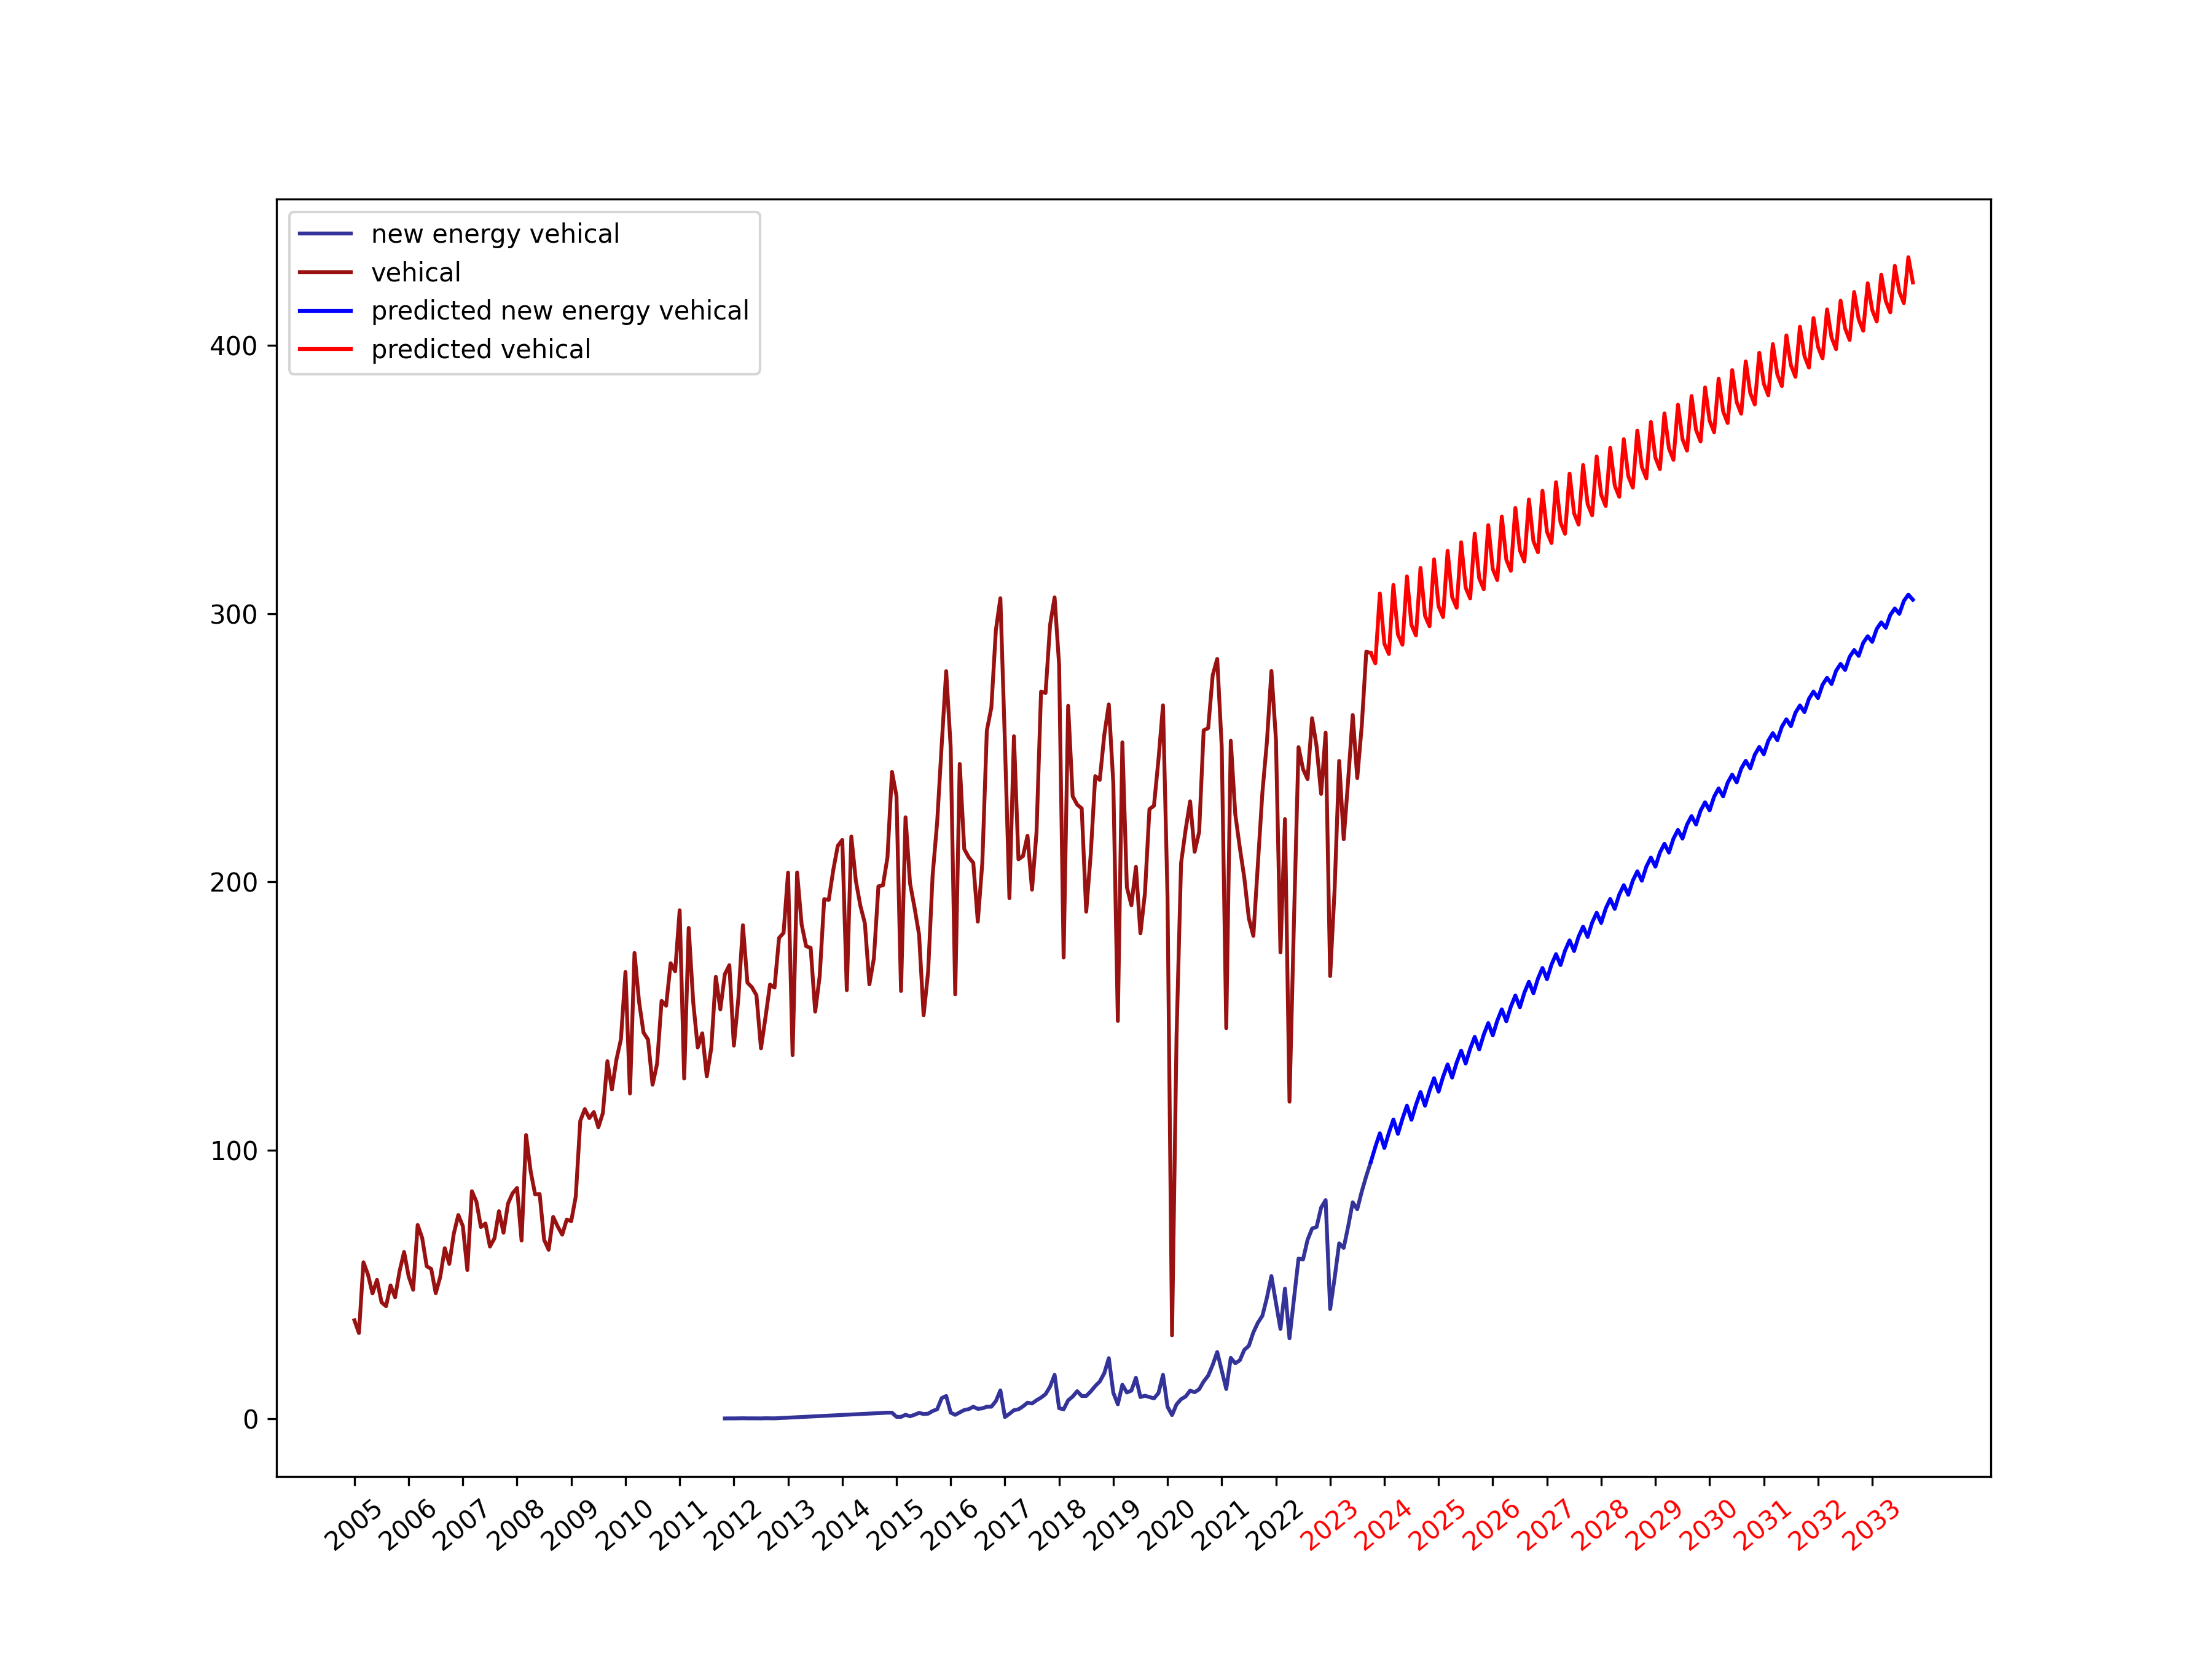
\includegraphics[width=30pc, height=22pc]{ARIMA_predict}
	\caption{ARIMA model prediction.}
	\label{figure 3}
\end{figure}

In Figure \ref{figure 3}, the red-highlighted years on the horizontal axis denote the forecasted results of the ARIMA model. If the line predicted by ARIMA is extended backward, it closely follows the trend of existing data points. Consequently, the model's forecasts are deemed to broadly adhere to the trends in both car sales and new energy electric vehicle sales.

From the forecasted results, it's evident that the growth rate of new energy electric vehicle sales surpasses that of total car sales. In other words, the proportion of new energy electric vehicles within the overall car market is increasing. This suggests that the development pace of new energy electric vehicles in China will be notably faster than that of traditional cars in the next ten years.


\subsection{Model for Question 3}

\subsubsection{Terms, Definitions and Symbols}

The Symbols used in this section will be demonstrated right following its use.

\subsubsection{Assumptions}

It is assumed that there exists a linear relationship between the sales of new energy electric vehicles and traditional cars in a short period. Additionally, we consider these two variables to be independent, thereby disregarding the identical influence that factors like household income might have on both variables. Finally, since the data we've collected is on a monthly basis, we consider both sets of data to represent continuous variables.

For the data we've collected, we assume that the automobile market is primarily composed of new energy electric vehicles and traditional cars, meaning the total car sales are the sum of new energy electric vehicle sales and traditional car sales.

\subsubsection{Data preparation}

We processed the previously collected data to obtain the sales figures for new energy electric vehicles and traditional cars. The data is displayed in Figure \ref{figure 4}.

\begin{figure}[htbp]
	\centering
	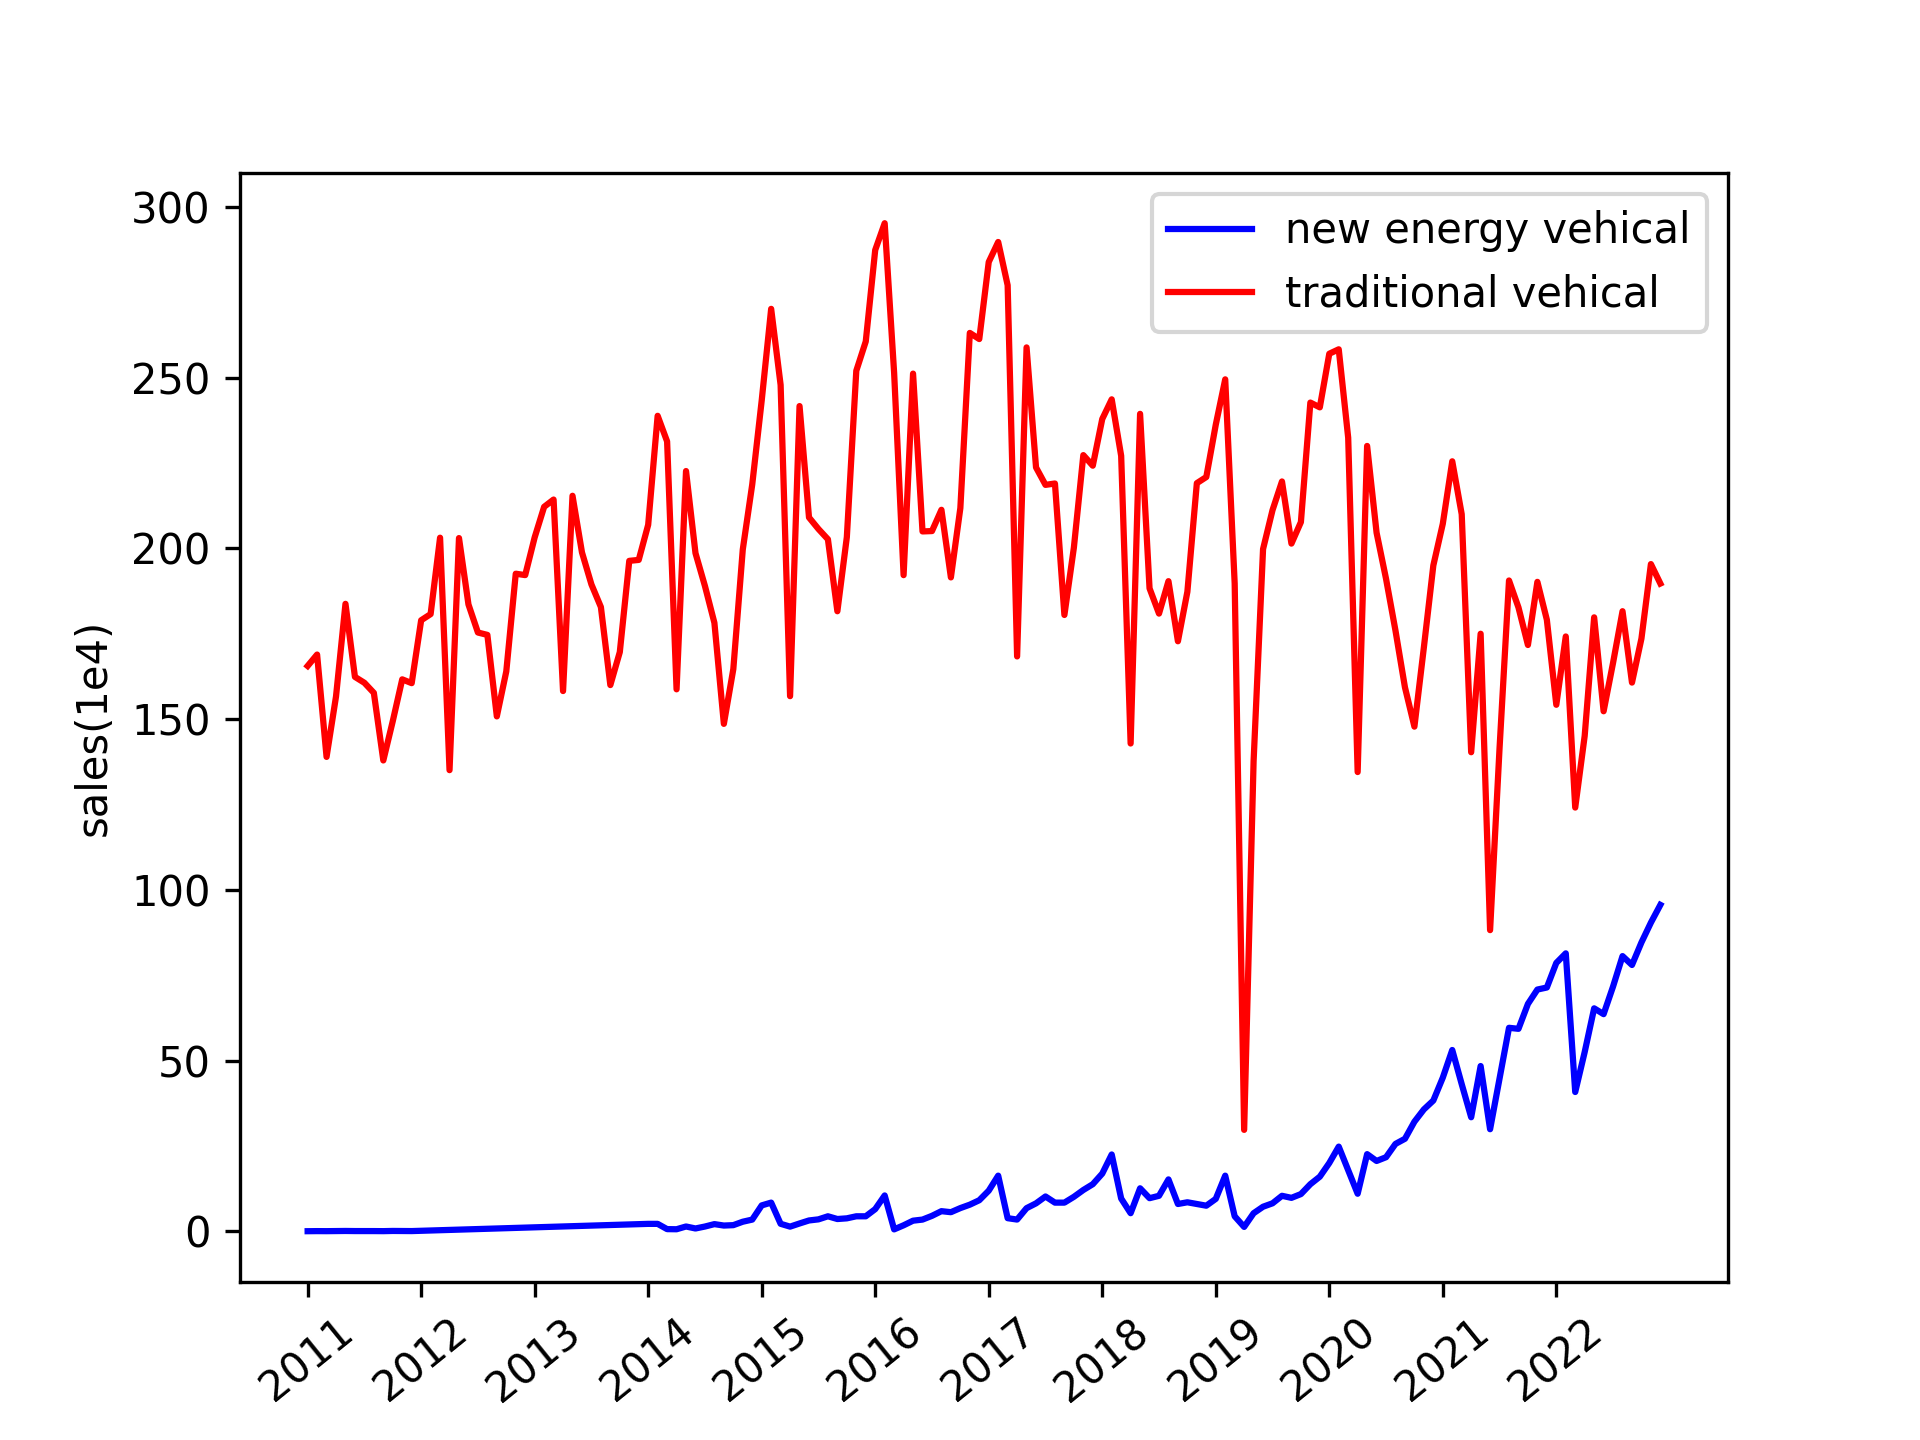
\includegraphics[width=30pc, height=22pc]{new_energy_and_tradition}
	\caption{Data of sales for for new energy electric vehicles and traditional cars.}
	\label{figure 4}
\end{figure}

\subsubsection{The Foundation and Solution of Model}

The modeling process of Pearson correlation is described as:

\textbf{Step1: }For the given inputs ${X}$ and ${Y}$, compute their sample means $\bar{X}$ and $\bar{Y}$ using the following formulas:

\begin{equation}
	\bar{X} = \frac{1}{n} \sum_{i=1}^{n} X_i \quad \text{; } \quad \bar{Y} = \frac{1}{n} \sum_{i=1}^{n} Y_i
\end{equation}

where $X_i$ means the $i$th sample in $X$, $Y_i$ means the $i$th sample in $Y$.

\textbf{Step2: }Calculate the sample covariance of variables $X$ and $Y$, indicating the overall strength and direction of the linear relationship between them. The formula for this step is as following:

\begin{equation}
	\text{Cov}(X, Y) = \frac{1}{n} \sum_{i=1}^{n} (X_i - \bar{X}) (Y_i - \bar{Y})
\end{equation}

where all symbols used are demontrated.

\textbf{Step3: }Calculate the sample standard deviations $\sigma_X$ and $\sigma_Y$ of variables X and Y respectively.

\begin{equation}
	\sigma_X = \sqrt{\frac{1}{n} \sum_{i=1}^{n} (X_i - \bar{X})^2} \quad \text{;} \quad \sigma_Y = \sqrt{\frac{1}{n} \sum_{i=1}^{n} (Y_i - \bar{Y})^2}
\end{equation}

\textbf{Step4: }Using the calculated mean, covariance, and standard deviation values, compute the Pearson correlation coefficient $\rho_{X,Y}$ between variables X and Y.

\begin{equation}
	\rho_{X,Y} = \frac{\text{Cov}(X, Y)}{\sigma_X \cdot \sigma_Y}
\end{equation}

The Pearson correlation coefficient measures the degree of linear relationship between two variables by dividing the covariance by their respective standard deviations. Its value ranges from -1 to 1, indicating both the strength and direction of the correlation between two variables. A coefficient close to 1 signifies a strong positive correlation, close to -1 indicates a strong negative correlation, and near 0 suggests little to no linear relationship between the two variables.


\subsubsection{Analysis of the Result}

Through our modeling, the computed Pearson correlation coefficient is approximately -0.1467. There exists a negative correlation between the sales of new energy electric vehicles and traditional cars. This implies that the development of new energy electric vehicles will have an impact on traditional car sales.

This result aligns with our forecast in the second question. In the second forecast, the growth rate of new energy electric vehicle sales outpaced that of all cars, indicating an increasing ratio between new energy vehicle sales and traditional car sales. This evidence collectively suggests a negative impact of new energy electric vehicles on the traditional automotive industry.




\section{Conclusions}



\subsection{Conclusions of the problem}



\subsection{Methods used in our models}



\subsection{Applications of our models}




\section{Future Work}

\subsection{Advanced models}
\% Optional.\CJK{UTF8}{gbsn}{ 如果希望模型完成更多功能,将期望的功能写在这里,当作对未来模型的展望。}

\subsubsection{model 1}

\subsection{Data collection}
\% Optional.\CJK{UTF8}{gbsn}{ 如果认为可以收集更多样化的数据,可以将期望的数据描述在这里。}

\subsubsection{data 1}




%参考文献
\begin{thebibliography}{9}%宽度9
\bibitem{1} Author, Title, Place of Publication: Press, Year of publication.
\bibitem{2} author, paper name, magazine name, volume number: starting and ending
page number, year of publication.

\end{thebibliography}

\newpage
%附录

\section{Appendix}

\begin{lstlisting}[caption={Data source}]

1. The brands of new energy electric vehicles that hold the largest market share.
http://cpcaauto.com/newslist.php?types=csjd&id=3273

\end{lstlisting}


\end{document} 